\definecolor{plot_orange}{rgb}{1, 0.639, 0}
\definecolor{plot_red}{rgb}{0.973, 0.463, 0.427}
\definecolor{plot_blue}{rgb}{0.153, 0.682, 0.937}
\definecolor{plot_green}{rgb}{0, 0.729, 0.22}
\definecolor{plot_gray}{rgb}{0.4, 0.4, 0.4}

In this chapter, we compare five different methods—Sparse, our SQL Einsum implementation, Torch, 
our Sparse Einsum, and our Legacy Sparse Einsum—on different problems. First, we compare them on 
various random tensor hypernetworks and then, we evaluate their performance on three instances of 
the ``Einsum Benchmark" \cite{einsum_benchmark} dataset.

\section{Random Tensor Hypernetworks}
To evaluate the performance of our implementations across a variety of properties that Einsum 
problems may exhibit, we generate Einsum expressions representing random tensor hypernetworks 
\cite{einsum_benchmark}, with each experiment featuring a single varying parameter. For every new 
parameter the results are evaluated using ten differently seeded random tensor hypernetworks 
generated with identical parameters. We then evaluate each methods performance on the problem 
ten times to get an average it/s.
\\
\\
First, we generate problems where we vary the maximum size of dimensions from 2 to 8. 
Figure \ref{fig:exp:max_dim_size} shows the performance for the different dimension sizes. 
The performance of all methods naturally decreases when the size of dimensions grows. However, 
the rate of this degradation differs significantly between the methods.

\begin{figure}[H]
    \centering
    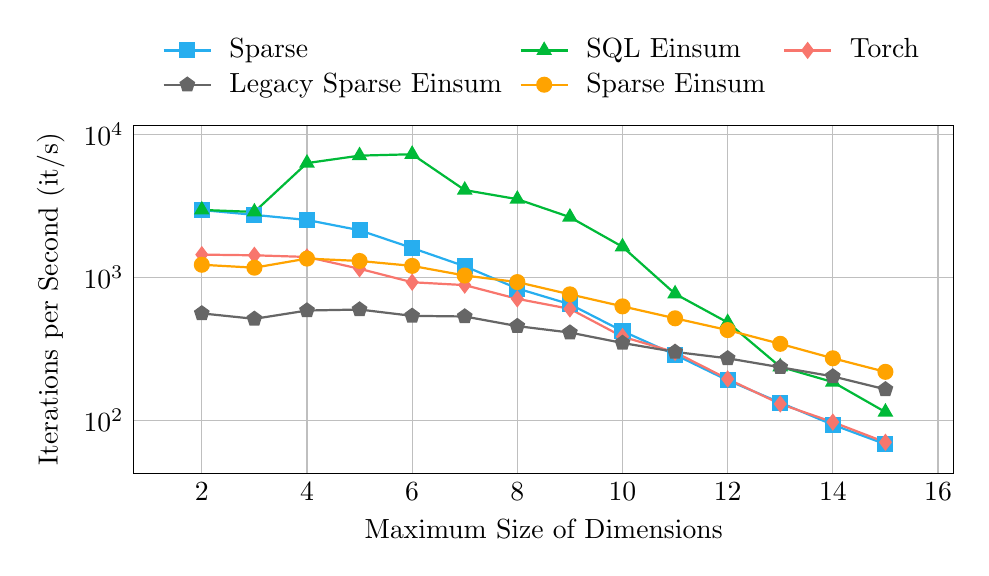
\begin{tikzpicture}
        \begin{semilogyaxis}[
            xlabel={Maximum Size of Dimensions},
            ylabel={Iterations per Second (it/s)},
            grid=major,
            mark size=2.5pt,
            width=12cm,
            height=6cm,
            enlargelimits=0.1,
            xtick style={draw=none},  % Remove x-axis tick marks
            ytick style={draw=none},  % Remove y-axis tick marks
            log basis y=10,           % Set base 10 for y-axis
            legend style={
                at={(0.5,1.05)}, % Position above the plot
                anchor=south, % Anchor to the south of the legend
                legend columns=3, % Arrange entries side by side
                column sep=1ex, % Space between columns
                draw=none, % Remove the border
                fill=none, % Remove the background fill
                legend cell align=left
            }
        ]
    
        % Sparse_Time (Square marker)
        \addplot[
            color=plot_blue,
            mark=square*,
            thick
        ] coordinates {
            (2, 2949.141) (3, 2728.197) (4, 2514.223) (5, 2130.835) 
            (6, 1600.128) (7, 1193.220) (8, 833.779) (9, 647.050)
            (10, 419.688) (11, 286.894) (12, 190.042) (13, 132.532)
            (14, 92.850) (15, 67.926)
        };
        \addlegendentry{Sparse}
    
        % SQL_Einsum_Time (Triangle marker)
        \addplot[
            color=plot_green,
            mark=triangle*,
            thick
        ] coordinates {
            (2, 2954.971) (3, 2861.648) (4, 6282.668) (5, 7085.857)
            (6, 7246.113) (7, 4068.557) (8, 3514.551) (9, 2631.675)
            (10, 1632.327) (11, 765.026) (12, 482.367) (13, 236.127)
            (14, 184.713) (15, 113.928)
        };
        \addlegendentry{SQL Einsum}
    
        % Torch_Time (Diamond marker)
        \addplot[
            color=plot_red,
            mark=diamond*,
            thick
        ] coordinates {
            (2, 1438.503) (3, 1422.954) (4, 1385.463) (5, 1145.090) 
            (6, 921.999) (7, 880.472) (8, 705.581) (9, 600.319)
            (10, 383.697) (11, 298.314) (12, 194.233) (13, 129.782)
            (14, 96.937) (15, 69.999)
        };
        \addlegendentry{Torch}
    
        % Legacy_Sparse_Einsum_Time (Pentagon marker)
        \addplot[
            color=plot_gray,
            mark=pentagon*,
            thick
        ] coordinates {
            (2, 558.216) (3, 511.409) (4, 584.589) (5, 594.116) 
            (6, 536.521) (7, 531.115) (8, 454.884) (9, 409.967)
            (10, 346.686) (11, 300.110) (12, 270.774) (13, 234.450)
            (14, 202.283) (15, 164.314)
        };
        \addlegendentry{Legacy Sparse Einsum}

        % Sparse_Einsum_Time (Circle marker)
        \addplot[
            color=plot_orange,
            mark=*,
            thick
        ] coordinates {
            (2, 1221.739) (3, 1165.713) (4, 1349.421) (5, 1298.878) 
            (6, 1199.998) (7, 1027.373) (8, 924.336) (9, 758.730)
            (10, 625.246) (11, 515.746) (12, 426.570) (13, 341.911)
            (14, 270.924) (15, 217.710)
        };
        \addlegendentry{Sparse Einsum}
    
        \end{semilogyaxis}
    \end{tikzpicture}
    \caption{Performance of different methods as a function of maximum dimension size. The plot shows the number of iterations per second for each method across varying dimension sizes.}
    \label{fig:exp:max_dim_size}
\end{figure}

\noindent
Sparse performance decreases quickly when the maximum number of dimensions that the tensors 
can have increases. It starts of with around the same it/s as SQL but declines faster than 
the other methods, coming in last with about the same performance as Torch. In general, 
SQL Einsum is superior for small till medium sizes of dimensions, but it also declines more 
steeply in comparison all other methods. The SQL implementations iterations per second rise, 
when the maximum size of dimensions increases from 2 to 6 and from thereon decreases constantly. 
Sparse Einsum and the legacy version of Sparse Einsum demonstrated very similar trends, 
though the legacy variant performed worse at all dimension sizes than the newer implementation. 
\\
\\
The results of Figure \ref{fig:exp:max_num_dim} illustrate how the computational performance 
of each method varies with increasing dimensionality in tensor hypernetworks. All of the methods
it/s decline as dimensionality increases, but start to flatten out at around nine. SQL Einsum 
starts of with by far the best performance, but declines rapidly, getting surpassed by Sparse Einsum 
and Legacy Sparse Einsum. Torch and Sparse perform about the same for higher number of dimensions, 
the only difference being that Sparse performs better than Torch for low numbers of dimensions. 
Overall, Sparse Einsum and Legacy Sparse Einsum handle the increasing dimensionality best, with 
Sparse Einsum displaying the highest iterations per second for problems with higher dimensionality. 

\begin{figure}[H]
    \centering
    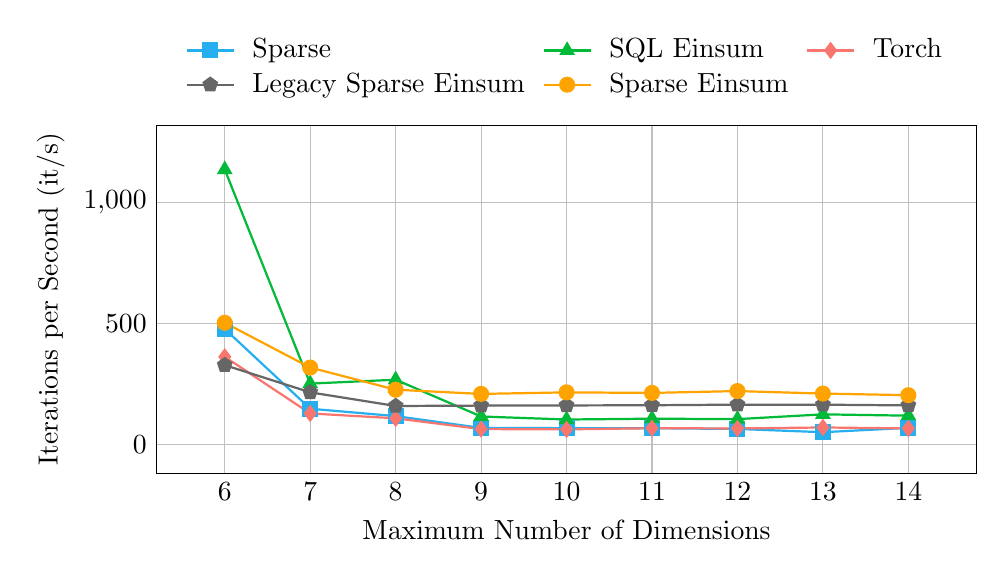
\begin{tikzpicture}
        \begin{axis}[
            xlabel={Maximum Number of Dimensions},
            ylabel={Iterations per Second (it/s)},
            grid=major,
            mark size=2.5pt,
            width=12cm,
            height=6cm,
            enlargelimits=0.1,
            xtick style={draw=none},  % Remove x-axis tick marks
            ytick style={draw=none},  % Remove y-axis tick marks
            ymin=0, ymax=1200,        % Set limits to ensure proper visualization
            legend style={
                at={(0.5,1.05)}, % Position above the plot
                anchor=south, % Anchor to the south of the legend
                legend columns=3, % Arrange entries side by side
                column sep=1ex, % Space between columns
                draw=none, % Remove the border
                fill=none, % Remove the background fill
                legend cell align=left
            }
        ]
    
        % Sparse_Time (Square marker)
        \addplot[
            color=plot_blue,
            mark=square*,
            thick
        ] coordinates {
            (6, 477.020) (7, 146.725) (8, 116.174) (9, 67.275) 
            (10, 66.349) (11, 65.991) (12, 62.998) (13, 49.544) (14, 67.529)
        };
        \addlegendentry{Sparse}
    
        % SQL_Einsum_Time (Triangle marker)
        \addplot[
            color=plot_green,
            mark=triangle*,
            thick
        ] coordinates {
            (6, 1136.583) (7, 250.692) (8, 266.833) (9, 114.571) 
            (10, 102.055) (11, 105.546) (12, 103.656) (13, 123.441) (14, 117.988)
        };
        \addlegendentry{SQL Einsum}
    
        % Torch_Time (Diamond marker)
        \addplot[
            color=plot_red,
            mark=diamond*,
            thick
        ] coordinates {
            (6, 361.691) (7, 127.232) (8, 107.009) (9, 62.497) 
            (10, 61.353) (11, 65.995) (12, 65.120) (13, 69.146) (14, 65.189)
        };
        \addlegendentry{Torch}
    
        % Legacy_Sparse_Einsum_Time (Star marker)
        \addplot[
            color=plot_gray,
            mark=pentagon*,
            thick
        ] coordinates {
            (6, 327.207) (7, 214.516) (8, 158.049) (9, 159.632) 
            (10, 160.321) (11, 161.135) (12, 163.633) (13, 163.505) (14, 160.476)
        };
        \addlegendentry{Legacy Sparse Einsum}

        % Sparse_Einsum_Time (Circle marker)
        \addplot[
            color=plot_orange,
            mark=*,
            thick
        ] coordinates {
            (6, 502.425) (7, 317.017) (8, 225.428) (9, 208.049) 
            (10, 214.421) (11, 212.171) (12, 219.846) (13, 209.382) (14, 202.798)
        };
        \addlegendentry{Sparse Einsum}
    
        \end{axis}
    \end{tikzpicture}
    \caption{Performance of different methods as a function of the maximum number of dimensions. The plot shows the number of iterations per second for each method.}
    \label{fig:exp:max_num_dim}
\end{figure}

\noindent
The plots in Figure \ref{fig:exp:num_tensors} show each method's performance as the number 
of tensors increases. Sparse starts off highest but declines sharply as the number of tensors 
grows, eventually becoming among the slowest methods. SQL Einsum is competitive at the start 
but also has a large drop-off. However, Torch displays stable performance, gradually 
decreasing but remaining more efficient at higher tensor counts than Sparse and SQL. 
Sparse Einsum and Legacy Sparse Einsum started of lower than the other methods but perform 
much better than the others as the number of tensors increases. Both Sparse Einsum versions 
end up with slightly more iterations per second than Torch for larger number of tensors. 
SQL and Sparse show by far the largest performance degradation.

\begin{figure}[H]
    \centering
    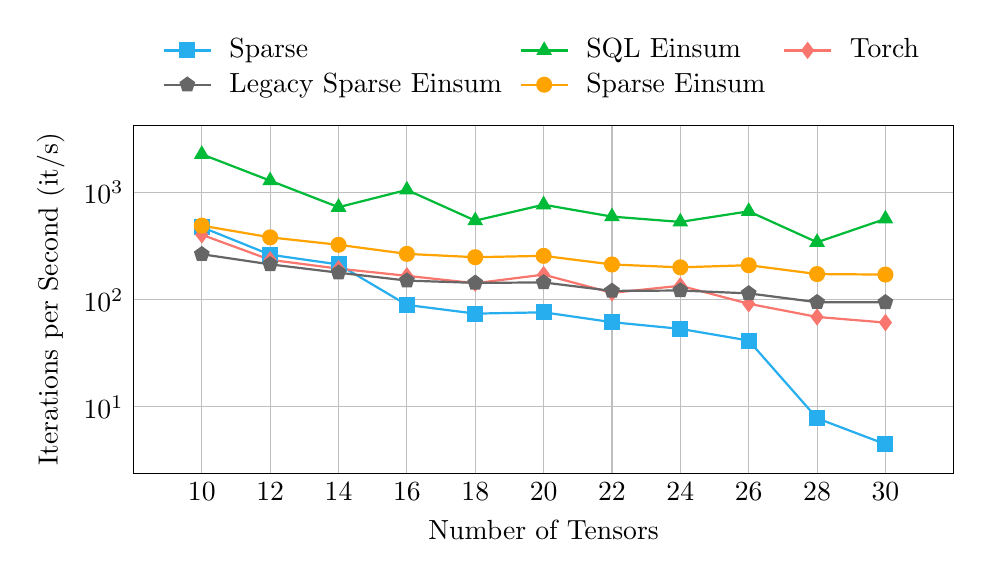
\begin{tikzpicture}
        \begin{semilogyaxis}[
            xlabel={Number of Tensors},
            ylabel={Iterations per Second (it/s)},
            grid=major,
            mark size=2.5pt,
            width=12cm,
            height=6cm,
            enlargelimits=0.1,
            xtick style={draw=none},
            ytick style={draw=none},
            xtick={10, 12, 14, 16, 18, 20, 22, 24, 26, 28, 30}, % Correct x-ticks
            xticklabels={10, 12, 14, 16, 18, 20, 22, 24, 26, 28, 30}, % Correct labels for x-ticks
            legend style={
                at={(0.5,1.05)}, % Position above the plot
                anchor=south, % Anchor to the south of the legend
                legend columns=3, % Arrange entries side by side
                column sep=1ex, % Space between columns
                draw=none, % Remove the border
                fill=none, % Remove the background fill
                legend cell align=left
            }
        ]
    
        % Sparse_Time (Square marker)
        \addplot[
            color=plot_blue,
            mark=square*,
            thick
        ] coordinates {
            (10, 476.545) (12, 263.609) (14, 213.613) (16, 89.564)
            (18, 74.276) (20, 76.383) (22, 61.785) (24, 53.520) 
            (26, 41.633) (28, 7.829) (30, 4.485)
        };
        \addlegendentry{Sparse}
    
        % SQL_Time (Triangle marker)
        \addplot[
            color=plot_green,
            mark=triangle*,
            thick
        ] coordinates {
            (10, 2284.108) (12, 1294.497) (14, 731.881) (16, 1061.477)
            (18, 548.178) (20, 772.391) (22, 597.661) (24, 533.237) 
            (26, 669.754) (28, 344.313) (30, 569.061)
        };
        \addlegendentry{SQL Einsum}
    
        % Torch_Time (Diamond marker)
        \addplot[
            color=plot_red,
            mark=diamond*,
            thick
        ] coordinates {
            (10, 404.718) (12, 236.199) (14, 195.213) (16, 167.394)
            (18, 142.753) (20, 171.697) (22, 116.004) (24, 135.279)
            (26, 91.784) (28, 69.143) (30, 61.248)
        };
        \addlegendentry{Torch}
    
        % Legacy_Sparse_Einsum_Time (Pentagon marker)
        \addplot[
            color=plot_gray,
            mark=pentagon*,
            thick
        ] coordinates {
            (10, 266.300) (12, 214.103) (14, 179.091) (16, 151.105)
            (18, 143.827) (20, 145.156) (22, 120.983) (24, 122.016) 
            (26, 114.738) (28, 94.909) (30, 94.717)
        };
        \addlegendentry{Legacy Sparse Einsum}
        
        % Sparse_Einsum_Time (Circle marker)
        \addplot[
            color=plot_orange,
            mark=*,
            thick
        ] coordinates {
            (10, 492.369) (12, 382.741) (14, 326.109) (16, 268.279)
            (18, 249.704) (20, 257.161) (22, 213.647) (24, 200.779) 
            (26, 210.283) (28, 173.847) (30, 171.929)
        };
        \addlegendentry{Sparse Einsum}
    
        \end{semilogyaxis}
    \end{tikzpicture}
    \caption{Performance of different methods as a function of the number of tensors.}
    \label{fig:exp:num_tensors}
\end{figure}

Figure \ref{fig:exp:density} shows the trends for performance of the different methods with 
decreasing density. We decrease the same tensor hypernetworks density for each step. Some methods 
improve drastically as the density decreases, while others remain about the same. In particular, 
SQL Einsum shows a dramatic improvement with lower densities, quickly accelerating from low 
performance at high densities to exceptional performance at the sparsest levels, generating an
S-curve. Sparse Einsum Legacy and Sparse Einsum both exhibit strong performance improvements as density decreases. That being said, 
Sparse Einsum tends to perform better than its legacy Sparse Einsum variant, especially at 
lower densities. On the other hand, the Torch method is quite stable across different densities, 
only showing minor fluctuations as the density decreases. The same can also be said for the 
Sparse method, which shows very little change across the density spectrum. The contrast 
emphasizes that some methods perform much better on dense data, while others are specialized 
for sparse data; the efficiency gains grow more dramatic as the data gets sparser.

\begin{figure}[H]
    \centering
    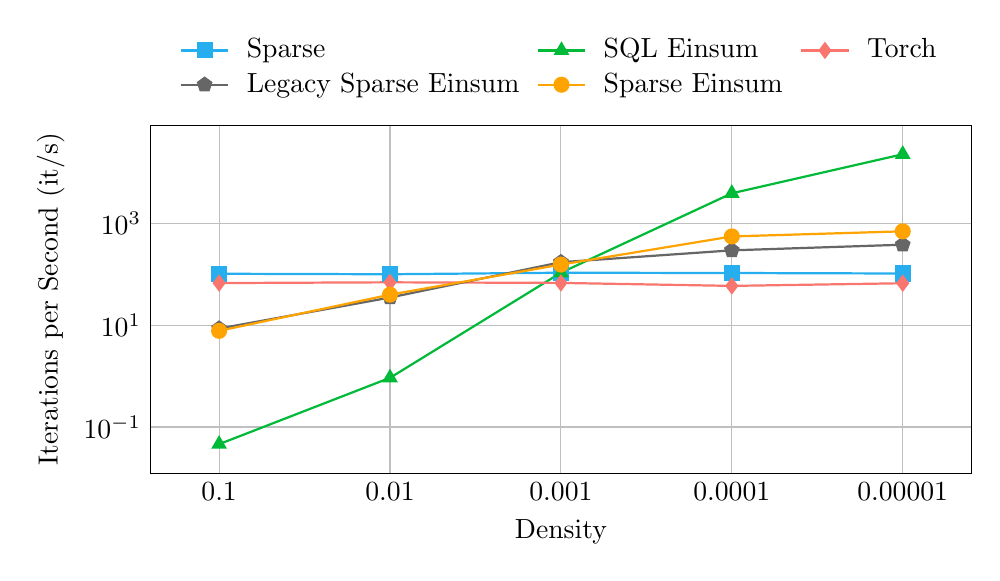
\begin{tikzpicture}
        \begin{semilogyaxis}[
            xlabel={Density},
            ylabel={Iterations per Second (it/s)},
            grid=major,
            mark size=2.5pt,
            width=12cm,
            height=6cm,
            enlargelimits=0.1,
            xtick style={draw=none},  % Remove x-axis tick marks
            ytick style={draw=none},  % Remove y-axis tick marks
            xtick={0.1, 0.01, 0.001, 0.0001, 0.00001}, % Specify custom x-axis ticks
            xticklabels={0.1, 0.01, 0.001, 0.0001, 0.00001}, % Set custom labels
            xmode=log,                % Logarithmic scale for x-axis
            log basis x=10,           % Set base 10 for x-axis
            x dir=reverse,
            legend style={
                at={(0.5,1.05)}, % Position above the plot
                anchor=south, % Anchor to the south of the legend
                legend columns=3, % Arrange entries side by side
                column sep=1ex, % Space between columns
                draw=none, % Remove the border
                fill=none, % Remove the background fill
                legend cell align=left
            }
        ]
    
        % Sparse_Time (Square marker)
        \addplot[
            color=plot_blue,
            mark=square*,
            thick
        ] coordinates {
            (0.1, 103.350) (0.01, 101.109) (0.001, 108.362) 
            (0.0001, 106.939) (0.00001, 104.600)
        };
        \addlegendentry{Sparse}
    
        % SQL_Time (Triangle marker)
        \addplot[
            color=plot_green,
            mark=triangle*,
            thick
        ] coordinates {
            (0.1, 0.046) (0.01, 0.929) (0.001, 108.230) 
            (0.0001, 3952.256) (0.00001, 23169.600)
        };
        \addlegendentry{SQL Einsum}
    
        % Torch_Time (Diamond marker)
        \addplot[
            color=plot_red,
            mark=diamond*,
            thick
        ] coordinates {
            (0.1, 67.884) (0.01, 70.186) (0.001, 68.328) 
            (0.0001, 59.668) (0.00001, 67.295)
        };
        \addlegendentry{Torch}
    
        % Sparse Einsum Legacy (Star marker)
        \addplot[
            color=plot_gray,
            mark=pentagon*,
            thick
        ] coordinates {
            (0.1, 8.646) (0.01, 35.231) (0.001, 174.506) 
            (0.0001, 298.441) (0.00001, 385.398)
        };
        \addlegendentry{Legacy Sparse Einsum}
        
        % Sparse_Einsum_Time (Circle marker)
        \addplot[
            color=plot_orange,
            mark=*,
            thick
        ] coordinates {
            (0.1, 7.789) (0.01, 40.1406) (0.001, 156.571) 
            (0.0001, 560.104) (0.00001, 706.623)
        };
        \addlegendentry{Sparse Einsum}

        \end{semilogyaxis}
    \end{tikzpicture}
    \caption{Performance comparison of different methods for varying densities on a logarithmic scale.}
    \label{fig:exp:density}
\end{figure}